\begin{frame}
    \frametitle{Entropy 2/3}
       \vspace*{-0.5cm}
  \begin{columns}[T]
  \small
    \begin{column}{0.5\textwidth}
        \begin{figure}
             \centering
             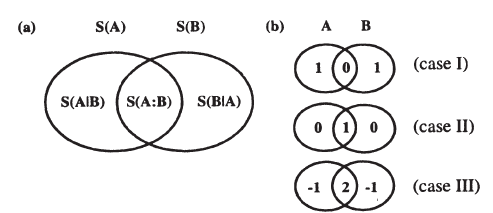
\includegraphics[width=1\textwidth]{gambar/DIAGRAM/diagram2.png}
             \captionsetup{font=tiny, justification=justified,width=1\textwidth}
             \captionof{figure}{(a) Diagram entropi umum untuk sistem komposit kuantum AB. (b) Diagram entropi untuk tiga kasus sistem 2 qubit: (I) independen, (II) terkorelasi secara klasik, (III) kuantum \textit{entanglement}.}
             \label{fig:EPR-Triplet}
        \end{figure}
        \begin{itemize} \tiny \justifying
        \vspace{-0.6 cm}
            \item Entropi von Neumann Persamaan \ref{Entropi von Neumann} diperkenalkan dalam mekanika kuantum, terkait dengan entropi Boltzmann-Gibbs-Shannon Persamaan \ref{entropi Boltzmann-Gibbs-Shannon} pada situasi klasik tertentu.
                \begin{equation}
                    S(p) = -\text{Tr}(p \log p)
                    \label{Entropi von Neumann}
                \end{equation}
                \begin{equation}
                    H(p) = -\sum_i P_i \log P_i
                    \label{entropi Boltzmann-Gibbs-Shannon}
                \end{equation}
                
        \end{itemize}
    \end{column}

   \begin{column}{0.5\textwidth}
        \begin{itemize} \tiny \justifying
           
                yang sesuai dengan sistem klasik \footcite{barnett2009quantum} yang berkorelasi.
            \item Entropy Negative\\
                Apabila memasukkan Persamaan \ref{density matrix AB} ke dalam Persamaan \ref{Entropi von Neumann} maka menghasilkan $S(A|B)=-1$. Persamaan conditional entropy dapat dituliskan sebagai
                \begin{equation}
                    S(A|B) \equiv S(AB) - S(B).
                \end{equation}
             \item Fungsi Negative Conditional Entropy\\
                Dalam konteks sistem kuantum komposit yang tidak diketahui, konsep entropi kondisional negatif terbukti sangat berguna dalam menjelaskan sistem kuantum yang terdiri dari beberapa bagian, serta memberikan pemahaman baru tentang pembentukan korelasi klasikal dari \textit{quantum entanglement} \cite{annur2022kepemilikan}.
        \end{itemize}
    \end{column}
  \end{columns}   
\end{frame}

\begin{frame}
    \frametitle{Entropy 3/3}
       \vspace*{-0.5cm}
  \begin{columns}[T]
  \tiny
    \begin{column}{0.5\textwidth}
\begin{align*}
\ket{\psi_{AB}} &= \frac{1}{2} (\ket{00} + \ket{11}){AB}. \\
\rho_{AB} &= \ket{\psi_{AB}}\bra{\psi_{AB}} \\
&= \frac{1}{2} (\ket{00} + \ket{11})_{AB} \otimes (\bra{00} + \bra{11}){AB}.\\
&= \frac{1}{2}(\ket{00}\bra{00}+\ket{00}\bra{11}+\ket{11}\bra{00}+\ket{11}\bra{11})\\
\hat{\rho}_A &= \text{tr}B (\rho{AB})\\
&= \frac{1}{2} \left( |0\rangle\langle 0|_A \text{tr} (|0\rangle\langle 0|_B) + |0\rangle\langle 1|_A \text{tr} (|0\rangle\langle 1|_B) \right. \\
& \quad + \left. |1\rangle\langle 0|_A \text{tr} (|1\rangle\langle 0|_B) + |1\rangle\langle 1|_A \text{tr} (|1\rangle\langle 1|_B) \right) \\
&= \frac{1}{2} (|0\rangle\langle 0|_A + |1\rangle\langle 1|_A) \\
&\equiv \frac{1}{2} I_A \\
\end{align*}
    \end{column}

   \begin{column}{0.5\textwidth}
   
\begin{align*}
\hat{\rho}_B &= \text{tr}_A(\rho_{AB}) \\
&= \frac{1}{2} \left[ \text{tr}(|0\rangle\langle 0|_A) \cdot |0\rangle\langle 0|_B + \text{tr}(|0\rangle\langle 1|_A) \cdot |0\rangle\langle 1|_B \right. \\
& \quad + \left. \text{tr}(|1\rangle\langle 0|_A) \cdot |1\rangle\langle 0|_B + \text{tr}(|1\rangle\langle 1|_A) \cdot |1\rangle\langle 1|_B \right] \\
&= \frac{1}{2} (|0\rangle\langle 0|_B + |1\rangle\langle 1|_B) \\
&\equiv \frac{1}{2} I_B.\\
\hat{\rho}_A \otimes \hat{\rho}_B &= I_A \frac{1}{2} \otimes I_B \frac{1}{2} \\
&= I_{AB} \frac{1}{4} \\
&\equiv \frac{1}{4} (|00\rangle\langle00| + |01\rangle\langle01| + |10\rangle\langle10| + |11\rangle\langle11|).\\
S(\hat{\rho}_A) &= S(\hat{\rho}_B) = -2 \times \left(\frac{1}{2}\right) \log\left(\frac{1}{2}\right) \equiv 1.\\
S(\rho_A | \rho_B) &= S(\rho_{AB}) - S(\hat{\rho}_B) = 0 - 1 \equiv -1 \\
S(\rho_B | \rho_A) &= S(\rho_{AB}) - S(\hat{\rho}_A) = 0 - 1 \equiv -1.
\end{align*}

    \end{column}
  \end{columns}  
\end{frame}